\clearpage
\subsection{Summary of Dynamic Memory Allocation Concepts} % (fold)
\label{sub:dymanic_memory_summary}

This chapter has introduced a number of concepts related to working with pointers and performing dynamic memory allocation.

\begin{figure}[htbp]
   \centering
   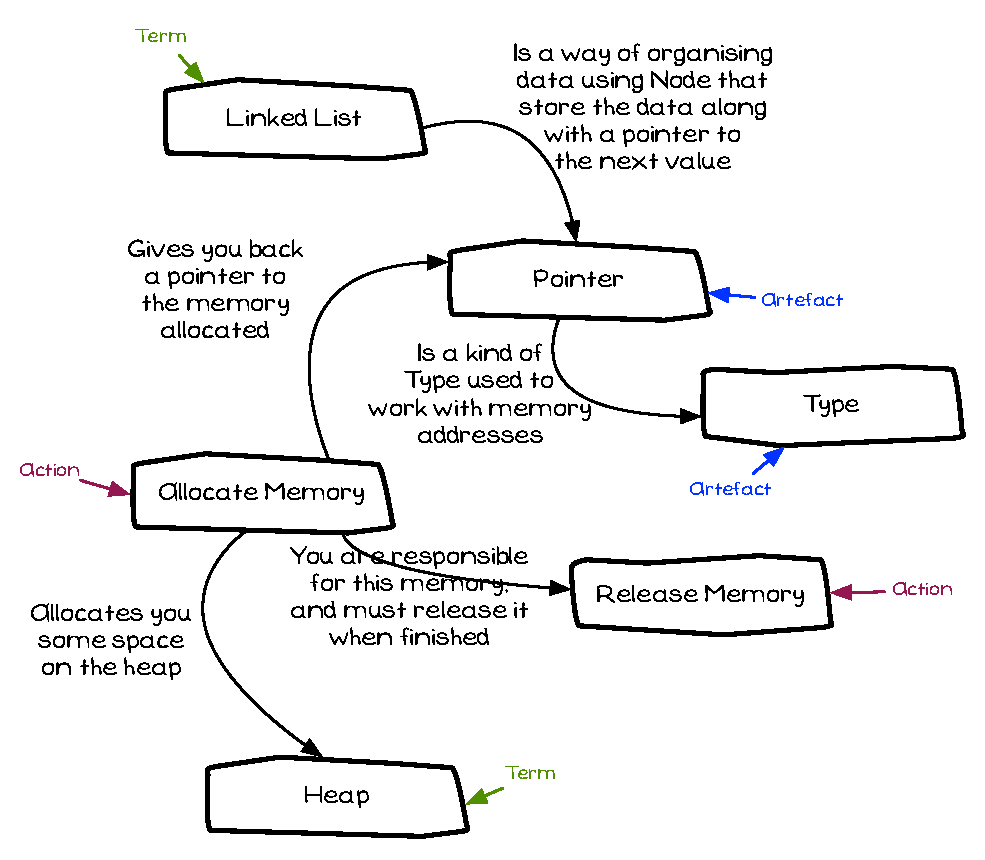
\includegraphics[width=0.9\textwidth]{./topics/dynamic-memory/diagrams/Summary} 
   \caption{Memory management focuses on allocating memory, releasing this allocation, pointers, and the heap}
   \label{fig:dynamic-memory-summary}
\end{figure}


\mynote{
\begin{itemize}
  \item \textbf{Heap} - an area of memory you can be allocated to store values.
  \item \textbf{Allocate Memory} - gives you ownership of a piece of the heap's memory.
  \item \textbf{Release Memory} - once you own the memory it is yours until it is released. If you forget to release it, it cannot be used by others.
  \item \textbf{Pointers} - are values that point to locations in memory. They store the address of the area of memory they refer to, and are needed to give you access to the heap.
\end{itemize}
}

% subsection summary (end)